
\chapter{Spectra}

%%%%%%%%%%%%%%%%%%%%%%%%%%%%%%%%%%%%%%%%%%%%%%%%%%%%%%%%%%%%%%%%%%%%%%%%%%%%%%%%%%%%%%%%%%
%%%%%%%%%%%%%%%%%%%%%%%%%%%%%%%%%%%%%%%%%%%%%%%%%%%%%%%%%%%%%%%%%%%%%%%%%%%%%%%%%%%%%%%%%%
\section{Introduction}
So, what are $\textit{spectral statistics}$? Do they have to do with rainbows? Sceptres? No, they don’t, but they’re almost as colorful and regal. The word spectral is borrowed from the spectral-like patterns observed in statistical physics - whether it may be atomic spectra or other quantum mechanical phenomena. The borrowing is loose and not literal, but still somewhat well founded. In fact, the field of Random Matrix Theory was extensively developed in the 1930s by the nuclear physicist Eugene Wigner. He found connections between the deterministic properties of atomic nuclei and their random and stochastic behaviors. The link? Random matrices.

So in the context of this thesis, $\textit{spectral statistics}$ will be an umbrella term for random matrix statistics that somehow involve that matrix's eigenvalues and eigenvectors. That being said, if we fix a $\textit{random matrix}$, we can study its features by studying its eigenvalues - fundemental numbers that tell us a lot about the matrix. They are quite important for many reasons. For instance in statistical physics, many processes are represented by operators or matrices, and as such, their behaviours could be partially determined by the eigenvalues of their corrosponding matrices. The study of eigenvalues and eigenvectors primarily falls in the scope of Linear Algebra, but their utility is far-reaching. So, what exactly are $\textit{eigenvalues}$ exactly?

%%%%%%%%%%%%%%%%%%%%%%%%%%%%%%%%%%%%%%%%%%%%%%%%%%%%%%%%%%%%%%%%%%%%%%%%%%%%%%%%%%%%%%%%%%

\subsection{The Quintessential Spectral Statistic: the Eigenvalue}
Given any standard square matrix $P \in \F^{N \times N}$, its \textit{eigenvalues} are simply the roots of the characteristic polynomial $\text{char}_P{(\lambda)}$ = $\det(P - \lambda I)$. By the Fundamental Theorem of Algebra, we know that there is always have as many complex eigenvalues $\lambda \in \Cc$ as the dimension of the matrix.

That being said, when our random matrix has a specified distribution (say, standard normal), we can see patterns in the eigenvalue distributions. So, an eigenvalue is a \textbf{spectral statistic} of a random matrix! To talk about a matrix's eigenvalues in a more formal and concise manner, we motivate what is the \text{eigenvalue spectrum}.

\newpage

\begin{definition}[Spectrum]
Suppose $P \in \F^{N \times N}$ is a square matrix of size $N$ over $\F$. Then, the (eigenvalue) spectrum of $P$ is defined as the multiset of its eigenvalues and it is denoted $\sigma(P) = \{\lambda_i  \in \Cc\}_{i=1}^N$. Note that it is important to specify that a spectrum is a multiset and not just a set; eigenvalues could be repeated due to algebraic multiplicity and we opt to always have $N$ eigenvalues.
\end{definition}

For example, consider the following code example from the RMAT package.
\begin{code}[Spectrum of a Standard Normal Matrix]
Let $P \sim \Normal(0,1)$ be a $4 \times 4$ standard normal random matrix. We can generate the spectrum of $P$, $\sigma(P)$ as follows:
\end{code}

\begin{lstlisting}[language=R]
library(RMAT)
P <- RM_norm(N = 5, mean = 0, sd = 1)
spectrum_P <- spectrum(P)
# Outputs the following
spectrum_P
...
        Re      Im   Norm Order
 1 -0.5434  1.3539 1.4589     1
 2 -0.5434 -1.3539 1.4589     2
 3  0.2255  1.4250 1.4427     3
 4  0.2255 -1.4250 1.4427     4
 5 -0.8678  0.0000 0.8678     5
\end{lstlisting}



While our definition for spectrum is nice and clean, there are a few caveats that we must take care of. First, how are spectra statistics? So we can even call them statistics, so there needs to be some formalization as to why we consider eigenvalues statistics. In this dialogue, we will call back on the same sort of formalization dialogue in the Random Matrices section. Before beginning, the reader is encouraged to review what a statistic is in the review appendix (A.x).

Recall that when we defined and motivated the $\D$-distribution framework of simulating random matrices,we always had one thing - a vector representation of random variables. Using this framework, the formalization is trivial.

\begin{remark}[Formalization]
Suppose $P \sim \D$ is an $N \times N$ random matrix. Then, $P$ has a representation as a sequence of $N^2$ random variables, denote it $\vec{X} = \{X_i \mid i = 1,2,\dots,N^2 - 1,N^2\}$. Then, the spectrum of the matrix $P$ is simply a function of the vector $\vec{X}$. We can denote this $\sigma(\vec{X})$, where the operator $\sigma$ is overloaded to mean the spectrum of a matrix $\textbf{with respect to the vector representation}$. The actual process for $\sigma$ is not necessary to explicitly write out, since characterizing it will be sufficient for now. Essentially, $\sigma$ is a function that would parse the random variables into the array form by index hacking. Then, it must compute the determinant of the matrix $P - \lambda I$, and solve for its roots. To summarize this, consider the flow chart below.
\end{remark}

To simplify the process, here is how we formalize the spectrum as a statistic. Suppose we sample $P \sim \D$. Then, we take its spectrum formally using $\sigma$ as such:\hfill
$$P_{\text{array}} \ra \vec{P} \ra \sigma(\vec{P}) \ra \text{index magic} \ra \det(P - \lambda I) \ra \sigma(P_{\text{array}})$$

%%%%%%%%%%%%%%%%%%%%%%%%%%%%%%%%%%%%%%%%%%%%%%%%%%%%%%%%%%%%%%%%%%%%%%%%%%%%%%%%%%%%%%%%%%

\subsection{Interlude: Ensembles}
While the spectrum of a matrix provides a good summary of the matrix, a matrix is only considered a single point/observation in random matrix theory. Additionally, simulating large matrices and computing their eigenvalues becomes harder and more computationally expensive as $N \to \infty$. As such, to obtain more eigenvalue statistics efficiently, another dimension is introduced by motiving the \textit{spectrum of a random matrix ensemble}.

\begin{definition}[Ensemble Spectrum]
If we have an ensemble $\Ens$, then we can naturally extend the definition of $\sigma(\Ens)$. To take the spectrum of an ensemble, simply take the union of the spectra of each of its matrices. In other words, if $\Ens = \{P_i \sim \mathcal{D} \mid P_i \in \F^{N \times N}\}_{i = 1}^K$, then $\sigma(\Ens) = \bigcup_{i=1}^K \sigma(P_i)$.
\end{definition}

For example, consider the following code example from the RMAT package.
\begin{code}[Spectrum of a Standard Normal Matrix Ensemble]
Let $\Ens \sim \Normal(0,1)$ be an ensemble of $3 \times 3$ standard normal random matrices of size $3$. We can generate the spectrum of $\Ens$, $\sigma(\Ens)$ as follows:
\end{code}

\begin{lstlisting}[language=R]
library(RMAT)
ens <- RME_norm(N = 3, mean = 0, sd = 1, size = 3)
spectrum_ens <- spectrum(ens)
# Outputs the following
spectrum_ens
...
        Re      Im   Norm Order
 1  1.7581  0.0000 1.7581     1
 2 -0.2614  1.0012 1.0347     2
 3 -0.2614 -1.0012 1.0347     3
 4  1.2327  0.4227 1.3032     1
 5  1.2327 -0.4227 1.3032     2
 6 -0.8504  0.0000 0.8504     3
 7 -0.5296  1.0508 1.1767     1
 8 -0.5296 -1.0508 1.1767     2
 9  0.7357  0.0000 0.7357     3
\end{lstlisting}

%****************************************************************************************
\begin{figure}[h]
 \begin{center}
  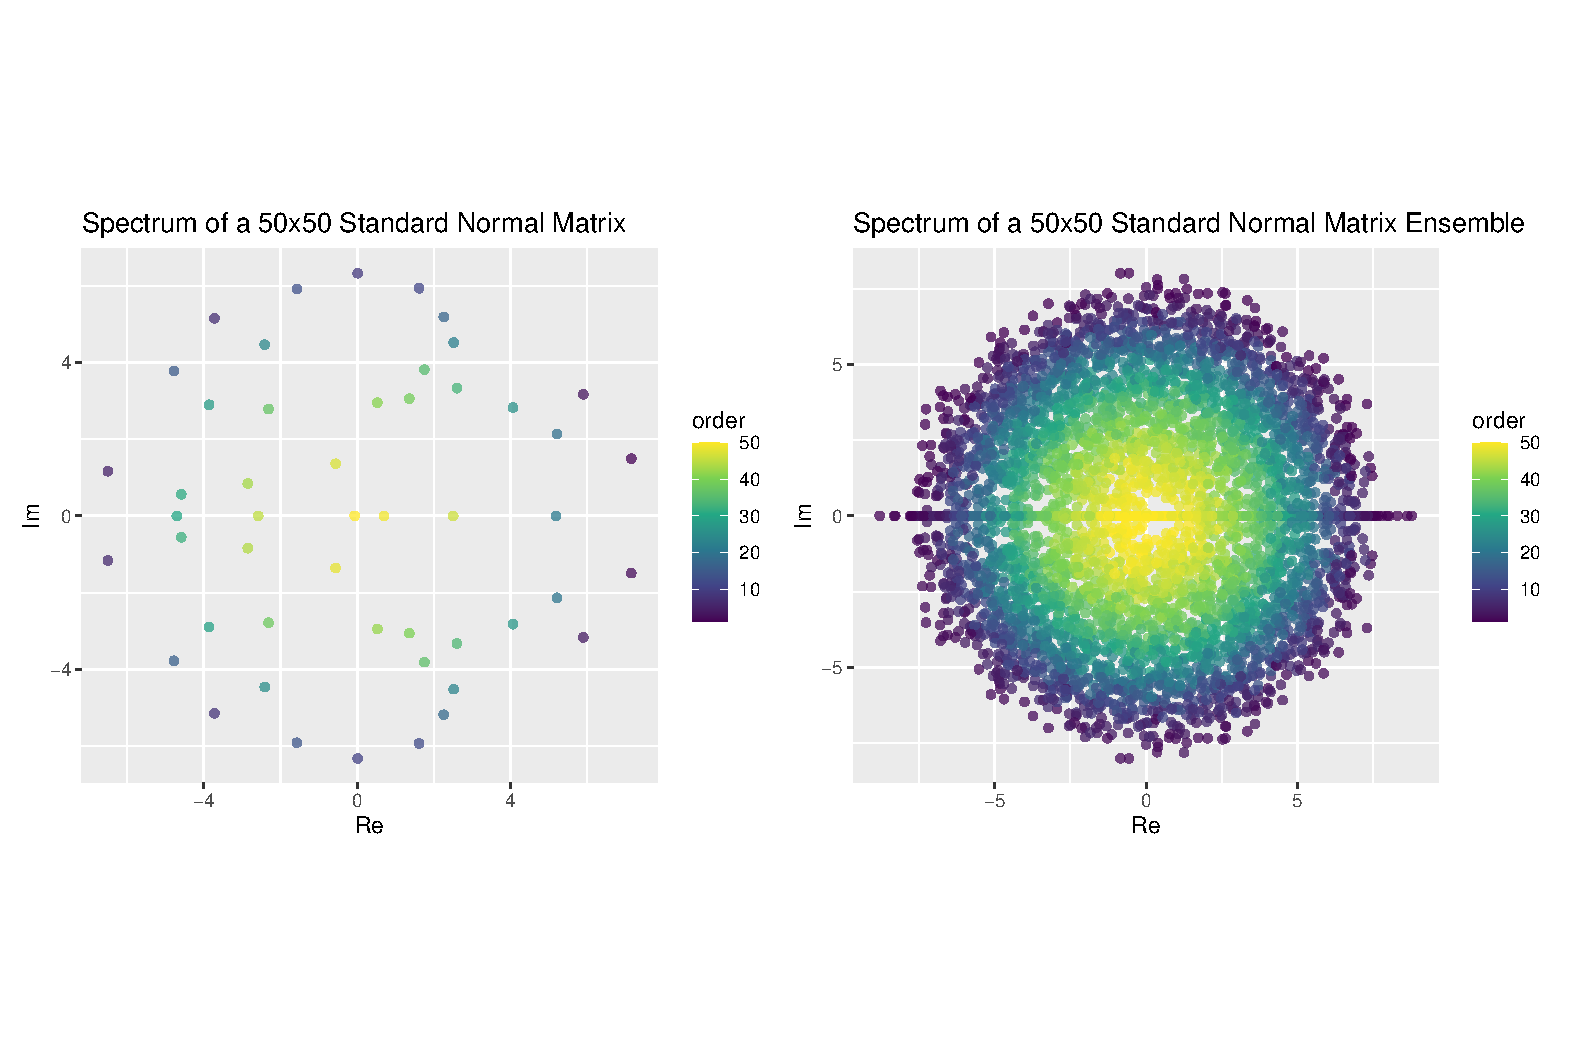
\includegraphics[scale = 0.7]{../graphics/chap2/2-1-2_comparison}
  \caption{Spectrum of a Beta Ensemble with the Sign-Ordered Scheme (Left) and Norm-Ordered Scheme (Right)}
 \end{center}
 \label{ensemble_comparison_plot}
\end{figure}
%****************************************************************************************

A common theme in this thesis will be that singleton matrices do not provide insightful information on their own. Rather, it is the collective behavior of a $\D$-distributed ensemble that tells us about how $\D$ impacts our spectral statistics. So in a way, ensemble statistics are the engine of this research.

%****************************************************************************************
\begin{figure}[h]
 \begin{center}
  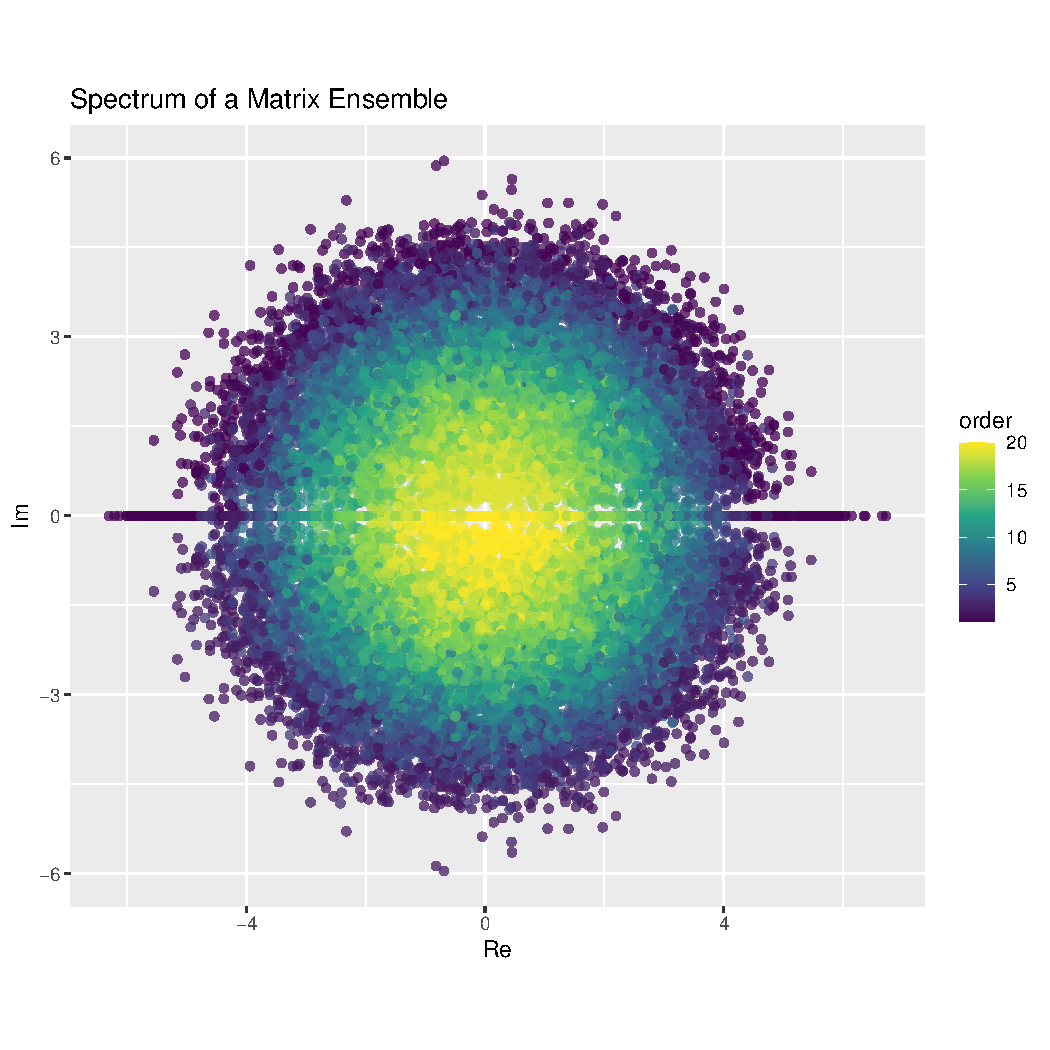
\includegraphics[scale = 0.7]{../graphics/chap2/2-1-2_normal_spec}
  \caption{Spectrum of a Standard Normal Matrix ensemble}
 \end{center}
 \label{spectrum_normal_ensemble_plot}
\end{figure}
%****************************************************************************************

%%%%%%%%%%%%%%%%%%%%%%%%%%%%%%%%%%%%%%%%%%%%%%%%%%%%%%%%%%%%%%%%%%%%%%%%%%%%%%%%%%%%%%%%%%
%%%%%%%%%%%%%%%%%%%%%%%%%%%%%%%%%%%%%%%%%%%%%%%%%%%%%%%%%%%%%%%%%%%%%%%%%%%%%%%%%%%%%%%%%%

\section{Ordered Spectra}

%%%%%%%%%%%%%%%%%%%%%%%%%%%%%%%%%%%%%%%%%%%%%%%%%%%%%%%%%%%%%%%%%%%%%%%%%%%%%%%%%%%%%%%%%%

\subsection{Eigenvalue Ordering}
When we motivate the idea of matrix dispersion in the next section, we will consider order statistics of that matrix's eigenvalues in tandem with its dispersion. However, to do so presupposes that we have a sense of what \textit{ordered} eigenvalues means. Take a matrix $P$ and its \textit{unordered} spectrum $\sigma(P) = \{\lambda_j\}$. It is paramount to know what ordering scheme $\sigma(P)$ is using, because otherwise, the eigenvalue indices are meaningless! So, to eliminate confusion, we add an index to $\sigma$ that indicates how the spectrum is ordered. Often, the ordering context will be clear and the indexing will be omitted. Consider the two following $\textit{ordering schema}$:

Standard definitions of an ordered spectrum follows the standard ordering in the reals; denote this as the ordering by the $\textbf{sign scheme}$. Note that because total-ordering is only well-defined on the reals, we can only use this scheme when on a spectrum with real entries. So, we write the $\textit{sign-ordered spectrum}$ as follows:
\begin{align*}
\sigma_S(P) = \{\lambda_j : \lambda_1 \geq \lambda_2 \geq \dots \geq \lambda_N\}_{j = 1}^N
\end{align*}
Alternatively, we can motivate a different scheme that properly handles complex eigenvalues. We could sort the spectrum by the norm of its entries; denote this as ordering using the \textit{norm scheme}. This way, all the eigenvalues are mapped to a real value, in which we could use the sign-scheme of ordering. Without further ado, we write the $\textit{norm-ordered spectrum}$ as follows:
\begin{align*}
\sigma_N(P) = \{\lambda_j : |\lambda_1| \geq |\lambda_2| \geq \dots \geq |\lambda_N|\}_{j = 1}^N
\end{align*}
Note that when we take the norms of the eigenvalues, we essentially ignore "rotational" features of the eigenvalues. Signs of eigenvalues indicate reflection or rotation, so when we take the norm, we essentially become more concerned with scaling.

For example, consider the following example.
\begin{center}
[Example showing the difference between the two schemes]
\end{center}

%****************************************************************************************
\begin{figure}[h]
 \begin{center}
  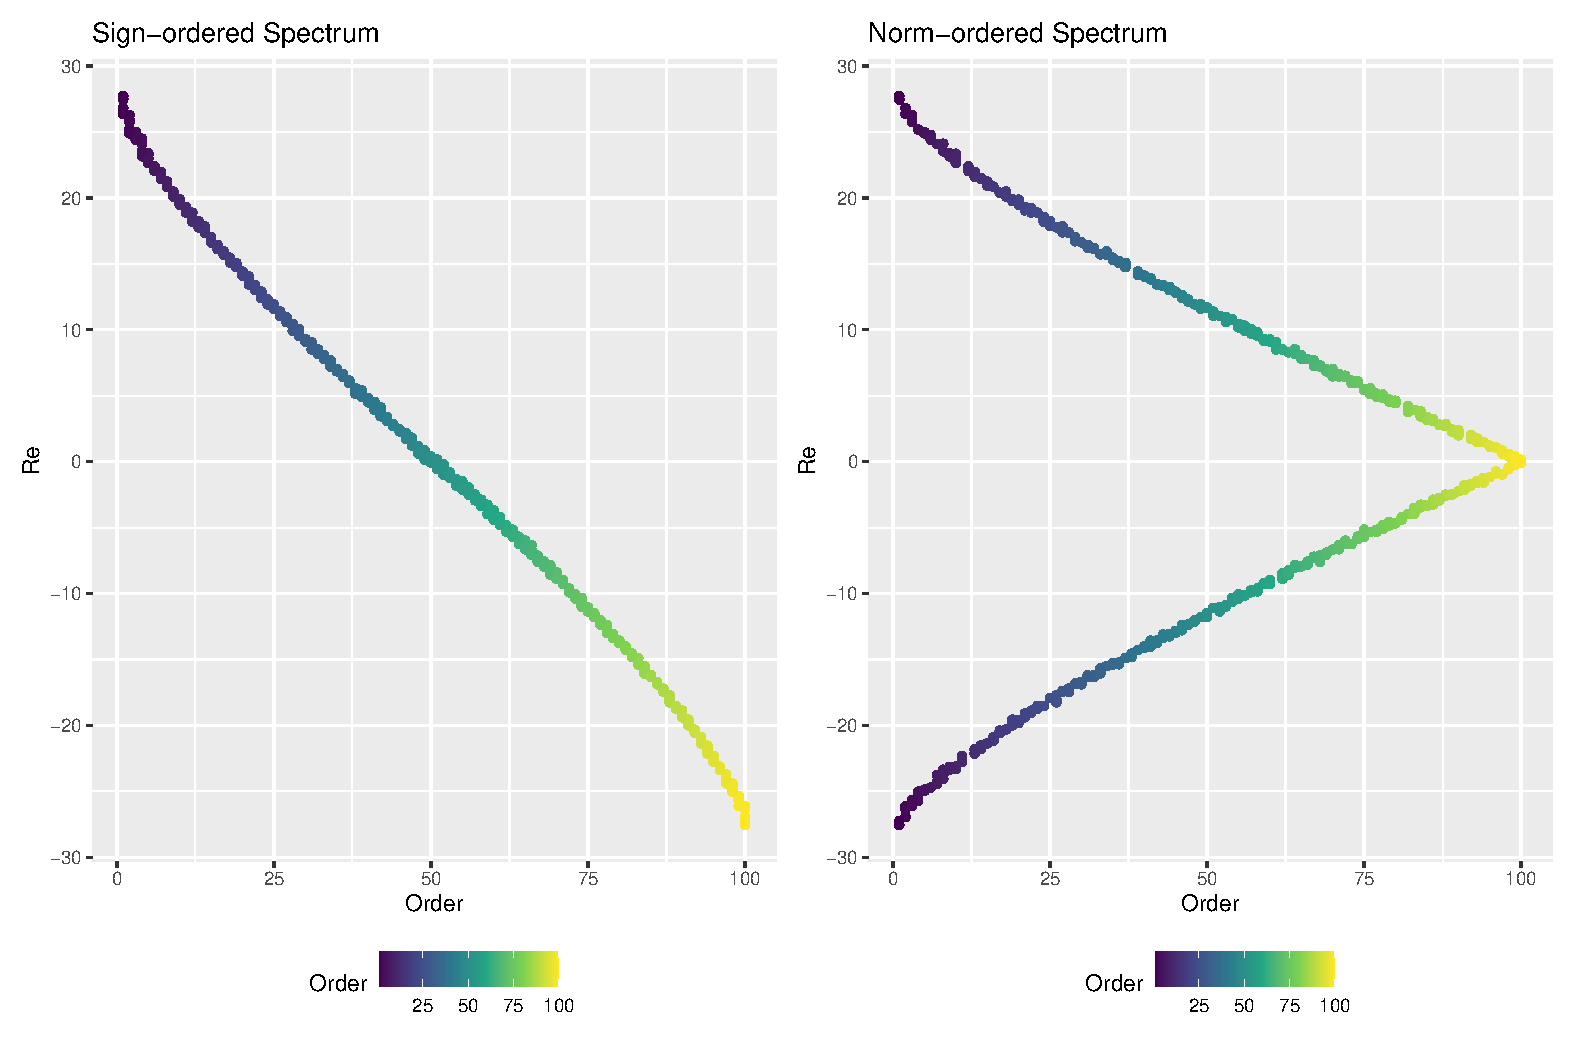
\includegraphics[scale = 0.7]{../graphics/chap2/2-2-1_orderscheme}
  \caption{Spectrum of a Beta Ensemble with the Sign-Ordered Scheme (Left) and Norm-Ordered Scheme (Right)}
 \end{center}
 \label{orderscheme_plot}
\end{figure}
%****************************************************************************************

%%%%%%%%%%%%%%%%%%%%%%%%%%%%%%%%%%%%%%%%%%%%%%%%%%%%%%%%%%%%%%%%%%%%%%%%%%%%%%%%%%%%%%%%%%
\newpage
\subsection{Singular Values}

An aternative to using the norm ordering scheme is using the singular values of the matrix. If a matrix is symmetric, the singular values are simply the norm of the eigenvalues. We ignore rotational features and focus solely on scale when we do so.

Suppose $P$ is a random matrix. Then, we can take it singular values as such.

\begin{definition}[Singular Values]
The singular values of a matrix $P$ are given by the square root of the eigenvalues of the corrosponding product of that matrix and its transpose. That is, $\sigma_+(P) = \sqrt{\sigma(P \cdot P^T)}$.
\end{definition}

\newpage
\begin{center}
$\textbf{Common Spectrum Schema}$
\end{center}

\spectrumschemetable

%%%%%%%%%%%%%%%%%%%%%%%%%%%%%%%%%%%%%%%%%%%%%%%%%%%%%%%%%%%%%%%%%%%%%%%%%%%%%%%%%%%%%%%%%%

\subsection{Order Statistics}

With eigenvalue ordering unambiguous and well-defined, we may proceed to start talking about their order statistics. In short, given a random sample of fixed size, order statistics are random variables defined as the value of an element conditioning on its rank within the sample. (See A.x)

In general, order statistics are quite useful and tell us a lot about how the eigenvalues distribute given a distribution. They tell us how the eigenvalues space themselves and give us useful upper and lower bounds.

For example, the maximum of a sample is an order statistic concerned with the highest ranked element. In our case, this could corrospond the largest eigenvalue of a spectrum. After all, a spectrum is a random sample of fixed size, so this statistic is well-defined.

\begin{example}[The Largest Eigenvalue]
Suppose we have seek the largest eigenvalue distribution for a ensemble distribution $\D$, we would simulate an ensemble $\Ens$ and observe $\lambda_1$ for each of its matrices. Then, we can set the distribution of the largest eigenvalue for $\D$ by observing the distribution of $\lambda_1$.
\end{example}

So, we fill consider the conditional order statistics $\E(\lambda_{i} \mid i)$ and $\Var(\lambda_{i} \mid i)$.

%%%%%%%%%%%%%%%%%%%%%%%%%%%%%%%%%%%%%%%%%%%%%%%%%%%%%%%%%%%%%%%%%%%%%%%%%%%%%%%%%%%%%%%%%%
%%%%%%%%%%%%%%%%%%%%%%%%%%%%%%%%%%%%%%%%%%%%%%%%%%%%%%%%%%%%%%%%%%%%%%%%%%%%%%%%%%%%%%%%%%

\section{Symmetric and Hermitian Matrices}

\subsection{Introduction}

A very important class of matrices in Linear Algebra is that of Symmetric or Hermitian matrices (See A.x). Simply put, those are matrices which are equal to their conjugate transpose.

$\textbf{Note:}$ Since real numbers are their own conjugate transpose, every Symmetric matrix is Hermitian. However, we will still delineate the two terms to avoid confusion.

In any case, one critical result in Linear Algebra that will be extensively wielded in this thesis is the fact that a matrix is Symmetric or Hermitian if and only if it has real eigenvalues. In other words:
\begin{align*}
P = \overline{P^{T}} \iff \sigma(P) = \{\lambda_i \mid \lambda_i \in \R\}
\end{align*}
Having a complete set of real eigenvalues yields many great properties. For instance, if all eigenvalues are real, we have the option of observing either the sign-ordered spectrum or the norm-ordered spectrum. This way, we can preserve negative signs and we would not lose the rotational aspect of the eigenvalue when we study its statistics. That is just one reason out of many more why having real eigenvalues is quite nice.

\subsection{Case Study: Wigner's Semicircle Distribution}

The eigenvalues of Hermitian matrices obey Wigner's Semicircle distribution. Since Hermitian matrices have real eigenvalues, then we can be more precise and generally say that the real component of the eigenvalues follow the semicircle distribution.

\begin{definition}[Semicircle Distribtion]
If a random variable $X$ is semicircle distributed with radius $R \in \R^+$, then we say $X \sim \text{SC}(R)$. $X$ has the following probability density function:
$$\Prb(X = x) = \frac{2}{\pi R^2} \sqrt{R^2 - x^2} \for x \in [-R, R]$$
\end{definition}


%****************************************************************************************
\begin{figure}[h]
 \begin{center}
  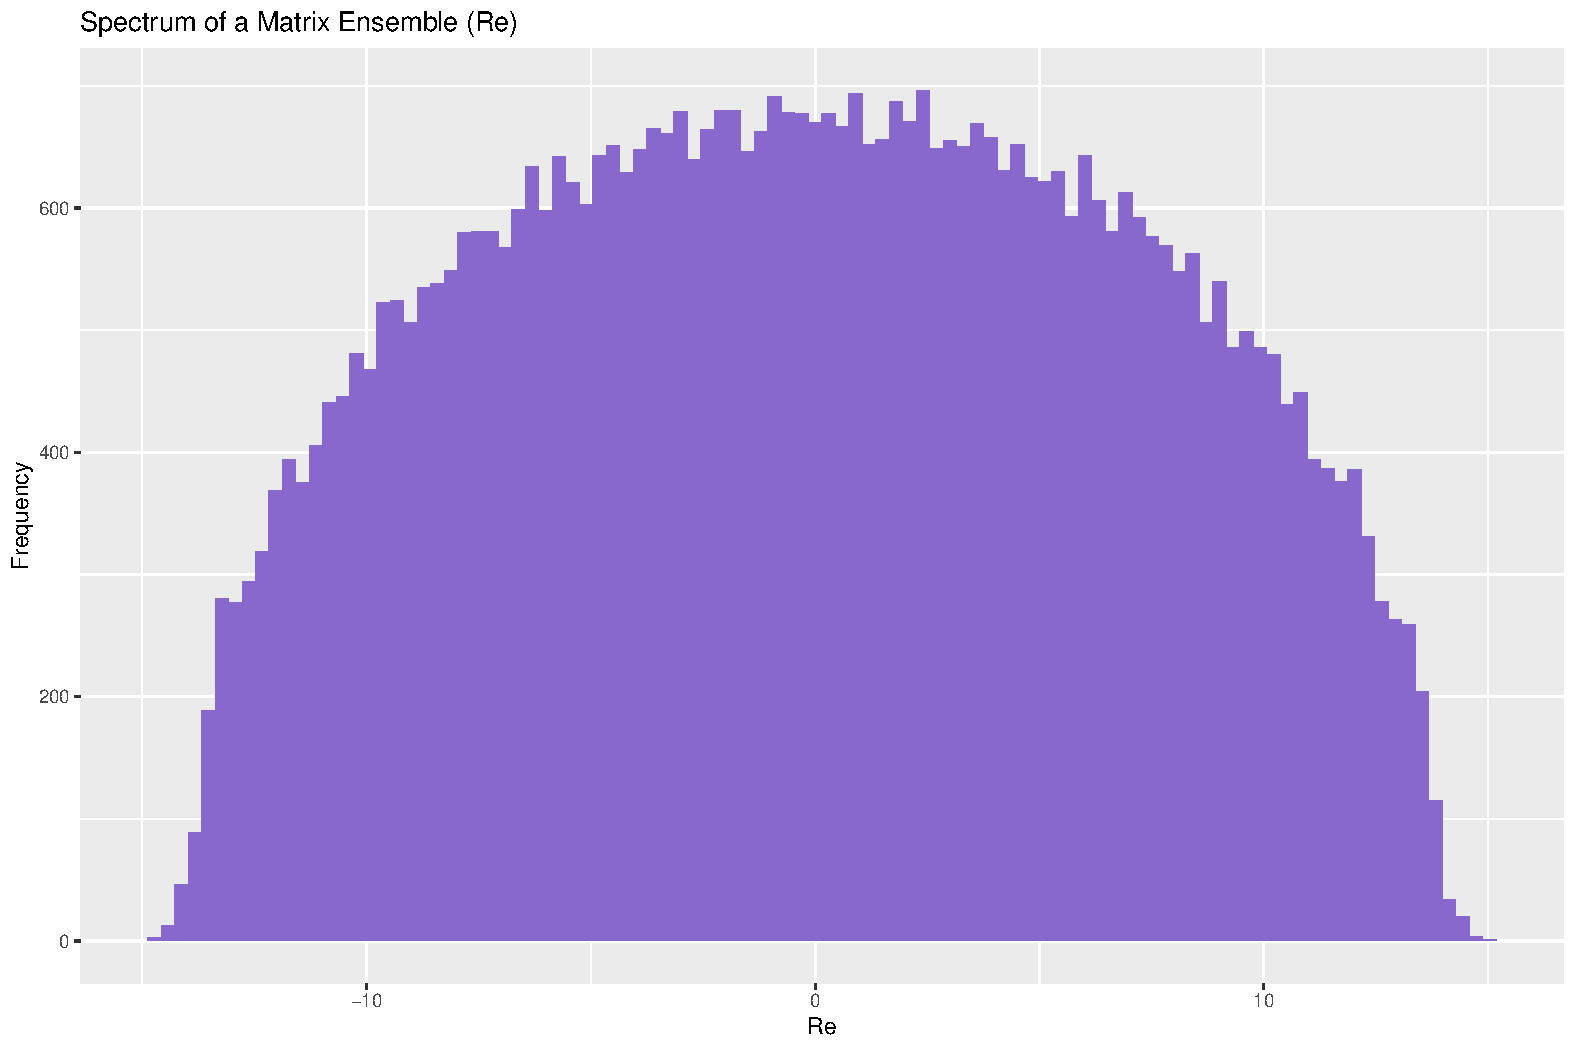
\includegraphics[scale = 0.7]{../graphics/chap2/2-3-2_semicircle}
  \caption{Dispersions of a $\beta = 4$ matrix with respect to ranking difference}
 \end{center}
 \label{semicircleplot}
\end{figure}
%****************************************************************************************

\begin{remark}[Radius and Matrix Dimension]
The dimension of the matrix determines the radius of the eigenvalues. Namely, if a Hermitian matrix $P$ is $N \times N$, then its eigenvalues are semicircle distributed with radius $R = 2\sqrt{N}$. That is, $P^{\dagger}$ has a spectrum $\sigma({P}) \sim \text{SC}(2\sqrt{R})$.
\end{remark}

%%%%%%%%%%%%%%%%%%%%%%%%%%%%%%%%%%%%%%%%%%%%%%%%%%%%%%%%%%%%%%%%%%%%%%%%%%%%%%%%%%%%%%%%%%
%%%%%%%%%%%%%%%%%%%%%%%%%%%%%%%%%%%%%%%%%%%%%%%%%%%%%%%%%%%%%%%%%%%%%%%%%%%%%%%%%%%%%%%%%%

%\section{Findings}
